\documentclass[12pt]{article}
\usepackage{amssymb,mathrsfs, amsmath,amsfonts}
\usepackage{mathtools}
\usepackage{graphicx}
\usepackage{enumitem}
\usepackage{braket}
\graphicspath{ {./ps3-assets/}{./exercises/handwritten/ps3/ps3-assets/} }

\title{Problem Set 3}
\author{CSE 468}
\date{\today}

\begin{document}

\maketitle



\begin{enumerate}[font=\bfseries]
    \item What is an operation we often use in our circuits that is \underline{not} unitary?
    \item \[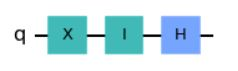
\includegraphics[scale=0.8]{single-q}\]
    Describe the above circuit as a single unitary matrix.
    \item \[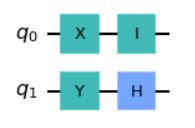
\includegraphics[scale=0.8]{double-q}\]
    Describe the above circuit as a single unitary matrix. Note: Qubit ordering is important here. Add example to clarify. (Follow Qiskit's notation)
    \item Why would we ever want to consider the tensor product of two gates?
    \item Write the below state as the tensor product of two qubits or prove it is an entangled state.
    \[\ket{\psi} = \frac{1}{\sqrt{2}}\ket{00} - \frac{i}{\sqrt{2}}\ket{01}\]
    \item Write the below state as the tensor product of two qubits or prove it is an entangled state.
    \[\ket{\psi} = \frac{1}{\sqrt{2}}\ket{01} + \frac{1}{\sqrt{2}}\ket{10}\]
    \item Give the statevector of each qubit system.
        \begin{enumerate}
            \item $\ket{10}$
            \item $\ket{0+}$
            \item $\ket{+-}$
        \end{enumerate}
    \item Give the parameters ($\theta,\phi,\lambda$) needed for the U gate to specify:
        \begin{enumerate}
            \item the Pauli X gate?
            \item the Pauli Y gate?
            \item the Pauli Z gate?
            \item the Hadamard gate?
        \end{enumerate}
    \item Consider the controlled-Y (CY) gate whose behavior is as follows: if the control bit is 0 it does nothing, if the control bit is 1 it applies the Pauli Y gate to the target bit. Give the matrix that describes the CY gate. Could we use this gate to create entanglement? Why or why not?
    \item Show the below equality is true. (See slide 15 of slide deck 9 for context)
    \[\frac{1}{\sqrt{2}}(\ket{01} - \ket{10}) = \frac{1}{\sqrt{2}}(\ket{+-} - \ket{-+})\]
    Remember quantum states are equivalent up to a common global phase.
    \item More questions about no cloning/entanglement?
\end{enumerate}



\end{document}